%HOW TO USE THIS DOCUMENT
%This template was created by Hammond Pearce
%  hammond.pearce@auckland.ac.nz
%by extending an existing template from Nathan Allen
%
%Load your bib file with the \addbibresource command 
%  (see immediately below these comments)
%Then,
% - A \footfullcite will put the citation at the 
%    bottom of the page
% - A \cite will not
% - Either way, citations are split up over reference slides
%     automagically at the end of the document
%     (it will create as many slides as necessary rather than 
%     having tiny fonts)
%You can use the existing introduction and results sections
%  as templates for content
%The existing slides also demonstrate different page layouts
%  e.g. one big picture, multiple columns, tables, etc
%
%Helpfully, this template creates section slides
%   The first slide that it creates has all sections visible
%   This is intended for the outline when presenting
%   Subsequent section break slides highlight the 
%      section title only

%Don't change: defines beamer class
\documentclass[compress,t,xcolor=table,dvipsnames]{beamer}

%Don't change: defines how to include the bibliography
\setbeamertemplate{bibliography item}{\insertbiblabel}
\usepackage[style=ieee,backend=bibtex,citetracker=true,doi=false,isbn=false]{biblatex}
\addbibresource{references.bib} 

%Don't change: these input the document preambles.
%You can change the preambles if you like (e.g. define
% additional macros, include more packages, etc)
\setbeamertemplate{bibliography item}{\insertbiblabel} %% Remove book symbol from references and add number


\let\oldcite=\cite             
\renewcommand{\cite}[1]{\textcolor[rgb]{1,0.3,0}{\oldcite{#1}}}

% See https://tex.stackexchange.com/a/396754/28146
\makeatletter
\newbibmacro*{hypercite}{%
  \renewcommand{\@makefntext}[1]{\noindent\normalfont##1}%
  \footnotetext{\scriptsize{%
    \textcolor[rgb]{1,0.3,0}{
    	\blxmkbibnote{foot}{%
	    \printtext[labelnumberwidth]{%
	      \printfield{prefixnumber}%
	      \printfield{labelnumber}}%
	}%
	\addspace
    \fullcite{\thefield{entrykey}}}}}}

\DeclareCiteCommand{\hypercite}%
  {\usebibmacro{cite:init}}
  {\usebibmacro{hypercite}}
  {}
  {\usebibmacro{cite:dump}}

% Redefine the \footfullcite command to use the reference number
\renewcommand{\footfullcite}[1]{\cite{#1}\hypercite{#1}}

\makeatother
\usepackage[LGR,T1]{fontenc}

\usepackage{pgf}
\usepackage{pgfplots,pgfplotstable}
\usepackage{tikz}
\usetikzlibrary{shapes,backgrounds}
\usetikzlibrary{arrows,shapes,fit,automata,positioning,decorations,calc}
\usetikzlibrary{spy,backgrounds}
\usepackage{siunitx}
\pgfplotsset{compat=1.12}
\usepackage{tabulary}
\usepackage{multirow}
\usepackage{appendixnumberbeamer}
\usepackage{booktabs}
\usepackage{listings}
\usepackage{subcaption}
\usepackage{graphicx}

%%%%%%%%%%%%%%%%%%%%%%For mathy things%%%%%%%%
\usepackage{mathtools}
\usepackage{amsmath}
\usepackage{amssymb}
\usepackage{amsthm}
\usepackage{amsfonts} %
\usepackage{calligra} %
%%%%%%%%%%%%%%%%%%%%%%%%%%%%%%%%%%%%%%%%%%%%%%%

% Media
\usepackage{multimedia}

\definecolor{graphFirst}{RGB}{2,136,209} % Light Blue 700
\definecolor{graphSecond}{RGB}{211,47,47} % Red 700
\definecolor{graphThird}{RGB}{245,124,0} % Orange 700
\definecolor{graphFourth}{RGB}{56,142,60} % Green 700
\definecolor{graphFifth}{RGB}{81,45,168} % Deep Purple 700
\definecolor{graphSixth}{RGB}{69,90,100} % Blue Grey 700
\definecolor{graphSeventh}{RGB}{251,192,45} % Yellow 700

\definecolor{backgroundFirst}{RGB}{129,212,250} % Light Blue 200
\definecolor{backgroundSecond}{RGB}{239,154,154} % Red 200
\definecolor{backgroundThird}{RGB}{255,204,128} % Orange 200
\definecolor{backgroundFourth}{RGB}{165,214,167} % Green 200
\definecolor{backgroundFifth}{RGB}{179,157,219} % Deep Purple 200
\definecolor{backgroundSixth}{RGB}{176,190,197} % Blue Grey 200
\definecolor{backgroundSeventh}{RGB}{255,245,157} % Yellow 200


\usepackage[linesnumbered]{algorithm2e}
\usepackage[scale=0.8,sfdefault,light]{roboto} 

\usetheme{Madrid}
\setbeamercovered{transparent}

\definecolor{uoa-blue}{RGB}{3,80,133}
\definecolor{uoa-light-blue}{RGB}{0,154,199}
\definecolor{uoa-grey}{RGB}{230,232,231}

\setbeamercolor{structure}{fg=uoa-blue}

\setbeamertemplate{blocks}[default]
\setbeamercolor{block title}{bg=uoa-blue,fg=white}
\setbeamercolor{block body}{bg=uoa-grey,fg=black}

\setbeamertemplate{title page}[default]

\setbeamertemplate{navigation symbols}{}
\setbeamertemplate{bibliography item}{\insertbiblabel}

\setbeamertemplate{itemize items}[default]
\setbeamertemplate{enumerate items}[default]

\setbeamertemplate{section in toc}[default]
\setbeamertemplate{subsection in toc}[default]

%\usepackage{fontspec}
%\defaultfontfeatures{Ligatures=TeX}
%\setromanfont{Verdana}


\setbeamercolor{normal text}{fg=black,bg=}
\setbeamercolor{alerted text}{fg=black,bg=}
\usebeamercolor{normal text}
\setbeamercovered{%
	again covered={\opaqueness<1->{15}}}

\newenvironment{myitemize}
{ \begin{itemize}
		\setlength{\itemsep}{6pt}     }
	{ \end{itemize}                  } 

\newenvironment{mypiecewiseitemize}
{ \begin{itemize}[<+>]
		\setlength{\itemsep}{6pt}     }
	{ \end{itemize}                  } 

\newenvironment{mycloseitemize}
{ \begin{itemize}
		\setlength{\itemsep}{3pt}     }
	{ \end{itemize}                  } 

\newenvironment<>{varblock}[2][\textwidth]{%
	\setlength{\textwidth}{#1}
	\begin{actionenv}#3%
		\def\insertblocktitle{#2}%
		\par%
		\usebeamertemplate{block begin}}
	{\par%
		\usebeamertemplate{block end}%
	\end{actionenv}}
	
	%\AtBeginSection[]
	%{
	%	\begin{frame}<beamer>
	%		\frametitle{Overview}
	%		\tableofcontents[currentsection]
	%	\end{frame}
	%
	
	\newenvironment{variableblock}[3]{%
		\setbeamercolor{block body}{#2}
		\setbeamercolor{block title}{#3}
		\begin{block}{#1}}{\end{block}}
	
	% Keys to support piece-wise uncovering of elements in TikZ pictures:
	% \node[visible on=<2->](foo){Foo}
	% \node[visible on=<{2,4}>](bar){Bar}   % put braces around comma expressions
	%
	% Internally works by setting opacity=0 when invisible, which has the 
	% adavantage (compared to \node<2->(foo){Foo} that the node is always there, hence
	% always consumes space plus that coordinate (foo) is always available.
	%
	% The actual command that implements the invisibility can be overriden
	% by altering the style invisible. For instance \tikzsset{invisible/.style={opacity=0.2}}
	% would dim the "invisible" parts. Alternatively, the color might be set to white, if the
	% output driver does not support transparencies (e.g., PS) 
	%
	\tikzset{
		invisible/.style={opacity=0},
		visible on/.style={alt={#1{}{invisible}}},
		alt/.code args={<#1>#2#3}{%
			\alt<#1>{\pgfkeysalso{#2}}{\pgfkeysalso{#3}} % \pgfkeysalso doesn't change the path
		},
	}
	
	\tikzset{onslide/.code args={<#1>#2}{%
			\only<#1>{\pgfkeysalso{#2}}
		}}
		\tikzstyle{highlight}=[red!90, fill=red!5]
		\tikzstyle{highlightsource}=[blue!90, fill=blue!5]
		\tikzstyle{borderhighlight}=[red!90, text=black, fill=red!5]
		\tikzstyle{texthighlight}=[text=red!90, fill=red!5]
\newcommand{\ignore}[1]{{}}

\newcommand{\bbb}{\mathbb{B}}
\newcommand{\bbn}{\mathbb{N}}
\newcommand{\bbr}{\mathbb{R}}
\newcommand{\Rnn}{{\bbr}_{\geq 0}}
\newcommand{\calL}{{\mathcal L}}
\newcommand{\calP}{{\mathcal P}}
\newcommand{\calA}{{\mathcal A}}
\newcommand{\exec}{\mathit{exec}}
\newcommand{\true}{\ensuremath{\mathsf{true}}}
\newcommand{\false}{\ensuremath{\mathsf{false}}}
\newcommand{\pref}{\preccurlyeq}
\newcommand{\sem}[1]{[\![#1]\!]}

\newcommand{\red}[1]{{\color{red}#1}}

\newcommand{\efalgo}{\ensuremath{{E_{\varphi}^*}}}
\newcommand{\ef}{\ensuremath{E_{\varphi}}}

\newcommand{\ptick}{\mathsf{ptick}}

\newcommand{\editI}{\mathsf{editI_{\varphi_I}}}
\newcommand{\editO}{\mathsf{editO_{\varphi}}}
\newcommand{\editIaut}{\mathsf{editI_{\calA_{\varphi_I}}}}
\newcommand{\editOaut}{\mathsf{editO_{\calA_\varphi}}}

\newcommand{\manEditI}{\mathsf{{man}\mbox{-} editI_{\varphi_{I}}}}
\newcommand{\manEditO}{\mathsf{{man}\mbox{-} editI_{\varphi_{O}}}}
\newcommand{\manEditIaut}{\mathsf{{man}\mbox{-} editI_{\calA_{\varphi_{I}}}}}
\newcommand{\manEditOaut}{\mathsf{{man}\mbox{-} editO_{\calA_\varphi}}}

\newcommand{\randEditI}{\mathsf{{rand}\mbox{-} editI_{\varphi_{I}}}}
\newcommand{\randEditO}{\mathsf{{rand}\mbox{-} editO_{\varphi}}}
\newcommand{\randEditIaut}{\mathsf{{rand}\mbox{-} editI_{\calA_{\varphi_{I}}}}}
\newcommand{\randEditOaut}{\mathsf{{rand}\mbox{-} editO_{\calA_\varphi}}}

\newcommand{\minEditI}{\mathsf{{minD}\mbox{-} editI_{\varphi_{I}}}}
\newcommand{\minEditO}{\mathsf{{minD}\mbox{-} editO_{\varphi}}}

\newcommand{\dist}{\mathsf{dist}}

\newcommand{\prefEditI}{\mathsf{{pref}\mbox{-} editI_{\varphi_{I}}}}
\newcommand{\prefEditO}{\mathsf{{pref}\mbox{-} editO_{\varphi}}}
\newcommand{\prefEditIaut}{\mathsf{{pref}\mbox{-} editI_{\calA_{\varphi_{I}}}}}
\newcommand{\prefEditOaut}{\mathsf{{pref}\mbox{-} editO_{\calA_\varphi}}}

\newcommand{\readInp}{\mathsf{read\_in\_chan}}
\newcommand{\readOut}{\mathsf{read\_out\_chan}}
\newcommand{\readPlant}{\mathsf{read\_plant\_chan}}
\newcommand{\readController}{\mathsf{read\_controller\_chan}}
\newcommand{\release}{\mathsf{release}}
%\texttt{ptick}

\newcommand{\okI}{\mathit{OK\_solutions_I}}
\newcommand{\okO}{\mathit{OK\_solutions_O}}

\newcommand{\bin}[1]{\overrightarrow{#1}}


\newcommand{\code}[1]{{\small{\texttt{#1}}}}
\newcommand\myeq{\stackrel{\mathclap{\normalfont\mbox{def}}}{=}}
% For definitions and Lemmas

%%%%%%%%%%%%%%%%%%%%%%%%%%%%%%%
	
% Don't change: this defines the environment for on-page footnote citations
\renewcommand\thefootnote{\textcolor{graphThird}{\arabic{footnote}}}

% Put your title here
\title[]{ Fast Hybrid System Simulation with Guaranteed Zero-crossing Detection }

% Put your author list here
\author[]{
	\large \textbf{Jin Woo Ro}
}

% Put your date here
\date[]{
	06/11/2019
}

% Put your institution and logo here
\institute[University of Auckland]
{
	
\includegraphics[scale=0.3]{fig/UOA-HC-RGB.png}
}

\begin{document}

%Don't change, this builds the outline slide
\frame{\titlepage}

% Problem and Objective slide:


%Include your introduction slides
\begin{frame} \frametitle{ Hybrid System Simulation }
	\vspace{-5pt}
	\begin{block}{Continuous Behaviour}
		\begin{myitemize}
			\item Continuous behaviour is captured using \textbf{ODEs}.
			\item Use \textbf{numerical methods} to solve ODEs.
			\begin{itemize}
				\item \textbf{Runge-Kutta (RK45)} is dominantly used
				\item Taylor, Euler, QSS, etc.
			\end{itemize}
		\end{myitemize}
	\end{block}
	
	\begin{block}{Discrete Behaviour}
		\begin{myitemize}
			\item Discrete behaviour is captured as discontinuity.
			\item Use \textbf{zero-crossing algorithms} to detect discontinuous points.
			\begin{itemize}
				\item {Bracket method} is used by Simulink.
				\item {Bisection method} is used by OpenModelica.
			\end{itemize}
		\end{myitemize}
	\end{block}
\end{frame}


\begin{frame} \frametitle{ Simulation Requirements }
	\vspace{-5pt}
	\begin{myitemize}
		\item Cyber-Physical Systems (CPSs) are safety-critical hybrid systems
		\item These require precise simulation for validation
	\end{myitemize}
	
	\begin{block}{ Requirements }
		\begin{myitemize}
			\item \textbf{Bounded local truncation error (LTE)} in solving ODEs.
			\item \textbf{Guaranteed zero-crossing detection (ZCD)}. This should deal with: 
			\begin{itemize}
				\item Even number of zero-crossings
				\item Falling into complex plane 
				\item Touching the zero-line
			\end{itemize}
		\end{myitemize}
	\end{block}
	
	\begin{figure}
		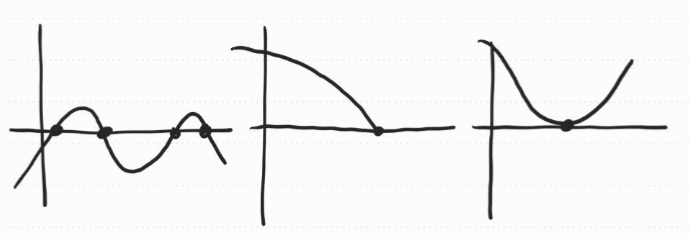
\includegraphics[width=0.6\textwidth]{./fig/zero-crossings.png}
	\end{figure}
	
\end{frame}

\begin{frame} \frametitle{RK45 (Fehlberg)}
	\vspace{-5pt}
	\begin{block}{Basic Idea}
		\begin{enumerate}
			\item Includes an adaptive step size algorithm
			\item $LTE = RK5(\Delta t) - RK4(\Delta t)$
			\item Increase/decrease the step size $\Delta t$ to control LTE
			\item Bounded LTE constraint: $|LTE| < tol$
		\end{enumerate}
	\end{block}
	
	\begin{block}{Limitation}
		\begin{enumerate}
			\item RK45 alone cannot do ZCD.
			\item Using root-finding algorithms with RK45 is theoretically possible, but will be extremely slow and can still miss ZCD.
		\end{enumerate}
	\end{block}
	\centering
\end{frame}

\begin{frame} \frametitle{Bracket/Bisection Methods}
	\vspace{-5pt}
	\begin{block}{Basic Idea}
		\begin{enumerate}
			\item Iterative approaches based on sign-change detection.
			\item Can be used with RK45.
		\end{enumerate}
	\end{block}
	
	\begin{block}{Limitation}
		\begin{enumerate}
			\item There must be a sign-change.
			\item Cannot handle challenging situations: 
			\begin{itemize}
				\item even number of zero-crossings
				\item complex plane
				\item touching the zero-line
			\end{itemize}
			\item Zero-crossing detection cannot be guaranteed.
		\end{enumerate}
	\end{block}
	\centering
\end{frame}

\begin{frame} \frametitle{ MQSS Methods }
	\vspace{-5pt}
	\begin{block}{Basic Idea}
		\begin{enumerate}
			\item In order to ensure zero-crossing detection, we proposed MQSS.
			\item Approximate each variable, and solve the guard.
			\item Using QSS-1 and QSS-2, two time solution $t1$ and $t2$ can be calculated.
			\item Ensure $|t1 - t2| < ttol$ by controlling $\Delta q$.
		\end{enumerate}
	\end{block}
	
	\begin{block}{Limitation}
		\begin{myitemize}
			\item Guard conditions have to be univariate
			\item Possibly slow solving due to many iterations needed to reach $|t1 - t2| < ttol$
			\item At stationary point $\dot{x} = 0$, there is no solution for $t$. Thus, the algorithm terminates unsuccessfully.
		\end{myitemize}
	\end{block}
	\centering
\end{frame}

\begin{frame} \frametitle{MQSS Finding the next time step }
	\centering
	\begin{figure} 
		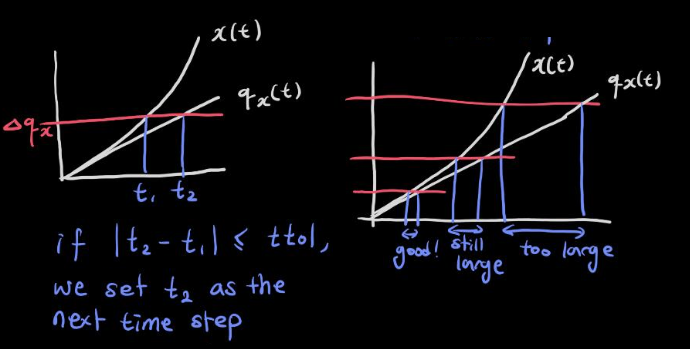
\includegraphics[width=1\textwidth]{./fig/dq1.png}
	\end{figure}
\end{frame}



\begin{frame} \frametitle{ Problem Statement }
	\begin{enumerate}
		\item Typical CPS models include multivariate nonlinear ODEs and guards.
		\item Precise simulation requires: 
			\begin{itemize}
			\item Bounded LTE
			\item Guarnateed ZCD
			\end{itemize}
		\item RK45 with Bracket/Bisection methods cannot guarantee ZCD.
		\item Recently proposed MQSS is accurate and can guarantee ZCD.
		\item However, MQSS has major limitations:
			\begin{itemize}
				\item Only allows univariate guards
				\item Simulation execution is slow
				\item Adaptive step size algorithm fails at stationary points
			\end{itemize}
		\item Thus, MQSS cannot simulate every CPS model.
		\item We need to overcome such limitations.
	\end{enumerate}
	
\end{frame}

\begin{frame} \frametitle{Contributions}
	\begin{myitemize}
		\item A new extension to HIOA, called HIOA/PD ( Hybrid Input Output Automata / Precomputed Differentiations )
		\item Compositional semantics including smooth-token exchange.
		\item A new algorithm for calculating the next time step.
		\item Comparison with existing methods.
	\end{myitemize}
\end{frame}

\begin{frame}[c] \frametitle{ Proposing idea brief description }

	\begin{enumerate}
		\item Convert the Simulink/Stateflow model into HIOA.
		\item This HIOA includes ODEs ($f$), update functions ($h$), and guards ($g$). These are all expressed as a function.
		\item By taking advantage of Sympy, precompute the differentiation for $f$, $h$, and $g$, up to the $\alpha$.
		\item Capture them in a new structure called HIOA/PD.
		\item Add smooth-tokens to allow exchange of derivative values between HIOA.
		\item For each continuous variable, we can obtain up to $n$th derivative value. Thus, we can approximate with $n$th order Taylor polynomials.
		\item Similarly, we compute I/O variables smooth-tokens.
		\item Finally, we can approximate $g$ using $n$th order Taylor polynomials. The only variable is $t$, so we can be solve it for $t$. Also, based on $g$, we set $\Delta q$.
	\end{enumerate}

\end{frame}

\begin{frame}[c] \frametitle{ Key Points }

	\begin{myitemize}
		\item We can guarantee that we always get at least one positive real root. This ensures that we always find delta values.
		\item We can guarantee that the found zero-crossing is always the first one. This ensures that we always correctly find zero-crossing.
		\item We can guarantee that the found solution $t$ is within the valid interval, which satisfies bounded LTE.
	\end{myitemize}

\end{frame}

\begin{frame}[c] \frametitle{ HIOA/PD Definition }
	\vspace{-5pt}
	\begin{block}{}
		$\mathcal{H} = \langle \alpha, L, X, V, O, Init, Inv, f, h, E, G, R\rangle $
		\begin{itemize}
		\item $\alpha \in \mathbb{N}_{\geq 1}$ is the maximum derivative order.
		\item $L = \{l_{0},\ldots,l_{n}\}$ a set of discrete locations.
		\item $X$ is a finite collection of continuous variable smooth-tokens. A smooth-token $x \in X$ is a sequence, $x = [ x^{(0)}, x^{(1)}, ..., x^{(\alpha)} ] $, where $x^{(n)} \in \mathbb{R}$ is $n$th derivative value. The domain of $X$ is $\mathbf{X} = \mathbb{R}^{n \times (\alpha + 1)}$, where $n$ is the number of continuous variables.
		\item $V$ is a finite collection of input variable smooth-tokens. For $v \in V$, $v$ is a sequence up to $\alpha$th derivative. The domain of $V$ is $\mathbf{V}$.
		\item $O$ is a finite collection of output variable smooth-tokens. For $o \in O$, $o$ is a sequence up to $\alpha$th derivative. The domain of $O$ is $\mathbf{O}$.
		\item $Init \subseteq \{l_0\} \times \mathbf{X} \times \mathbf{O}$.
		\item $Inv: \mathbf{L} \rightarrow 2^{\mathbf{X} \times \mathbf{V} }$
		\end{itemize}
	\end{block}
\end{frame}

\begin{frame}[c] \frametitle{ HIOA/PD Definition Cont. }
	\vspace{-5pt}
	\begin{block}{}
		\begin{itemize}
		
		\item $f : \mathbf{L} \times \mathbf{V} \times \mathbf{X} \times \mathbb{N}_{\geq 0,\leq \alpha} \rightarrow \mathbb{R}^{n}$ is a vector field for ODEs. E.g., 
		\begin{equation}
			f(l_0, V, X, 1) \myeq 
			\begin{bmatrix} 
				x^{(1)} \\
				y^{(1)} 
			\end{bmatrix}
			= 
			\begin{bmatrix} 
				\dot{x} \\
				\dot{y} 
			\end{bmatrix}
			=
			\begin{bmatrix}
				x \cos (y) \\
				x - y
			\end{bmatrix}
		\end{equation}
		\begin{equation}
			f(l_0, V, X, 2) \myeq 
			\begin{bmatrix} 
				x^{(2)} \\
				y^{(2)} 
			\end{bmatrix}
			= 
			\begin{bmatrix} 
				\ddot{x} \\
				\ddot{y} 
			\end{bmatrix}
			=
			\begin{bmatrix}
				-x \sin (y) \frac{dy}{dt} + \frac{dx}{dt} \cos (y) \\
				\frac{dx}{dt} - \frac{dy}{dt}
			\end{bmatrix}
		\end{equation}
		\item $h : \mathbf{L} \times \mathbf{X} \rightarrow \mathbf{O}$.
		\item $E \subset \mathbf{L} \times \mathbf{L} $ is a collection of discrete edges.
		\item $G : E \rightarrow 2^{\mathbf{X} \times \mathbf{V}}$ assigns to each
		  $e = (l, l') \in E$ a guard.
		\item
		  $R : E \times \mathbf{X} \times \mathbf{V} \rightarrow 2^{\mathbf{X} \times \mathbf{O}}$
		  assigns to each $e = (l,l') \in E$.
		\end{itemize}
	\end{block}
\end{frame}






\begin{frame}[c] \frametitle{ Main Example: cooperative robots }
	\begin{figure}
		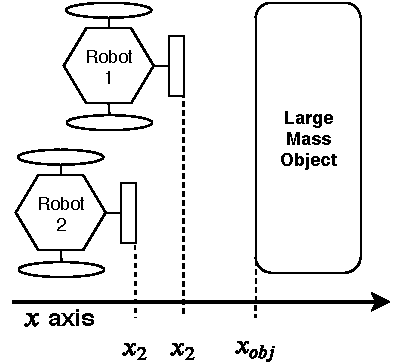
\includegraphics[width=0.45\textwidth]{./fig/diagrams/robots_diagram.pdf}
		\caption{A modified system presented in \footfullcite{chaimowicz2003hybrid}}
	\end{figure}
\end{frame}

\begin{frame}[c] \frametitle{ HIOA Model of cooperative robots }
	\begin{figure}
		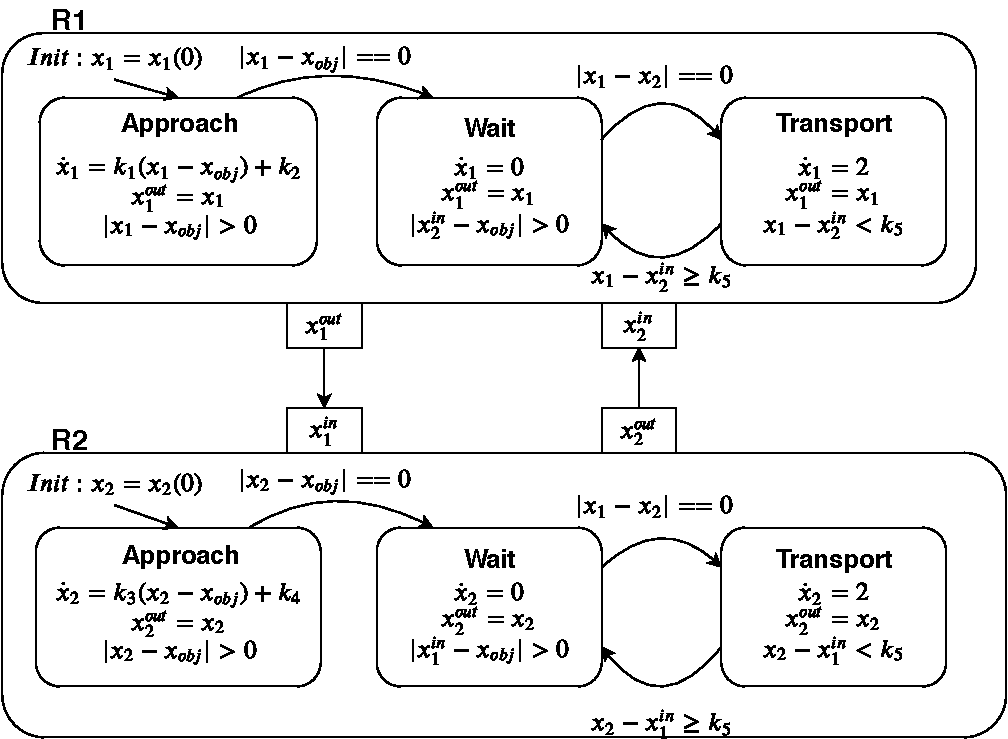
\includegraphics[width=0.7\textwidth]{./fig/diagrams/robots_ha.pdf}
		\caption{Hybrid automata model of cooperative robots. $k_1, k_2, k_3, k_4, k_5$, and $x_{obj}$ are constants. }
	\end{figure}
\end{frame}

\begin{frame}[c] \frametitle{ Other Example: Steeringwheel }
	\begin{figure}
		\centering
		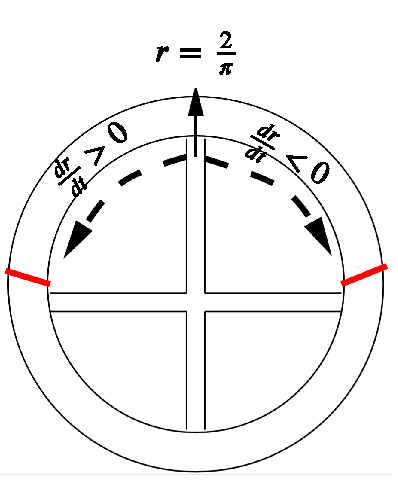
\includegraphics[width=0.4\textwidth]{./fig/diagrams/steeringwheel.pdf}
		\caption{Steeringwheel example in \footfullcite{ro2019compositional}}
	\end{figure}
\end{frame}

\begin{frame}[c] \frametitle{ Other Example: Two-tank }
	\begin{figure}
	\centering
	\begin{subfigure}{.4\textwidth}
	  \centering
	  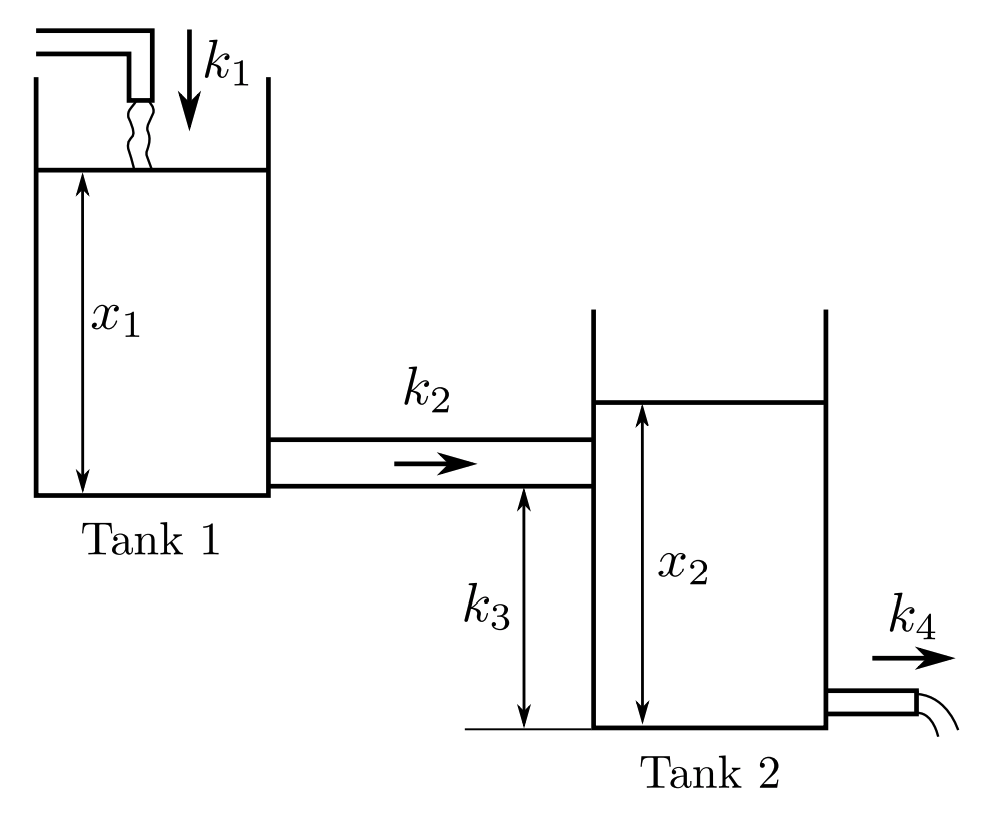
\includegraphics[width=0.8\textwidth]{./fig/diagrams/two-tank-diagram.png}
	  \caption{Physical setup}
	\end{subfigure}%
	\begin{subfigure}{.6\textwidth}
	  \centering
	  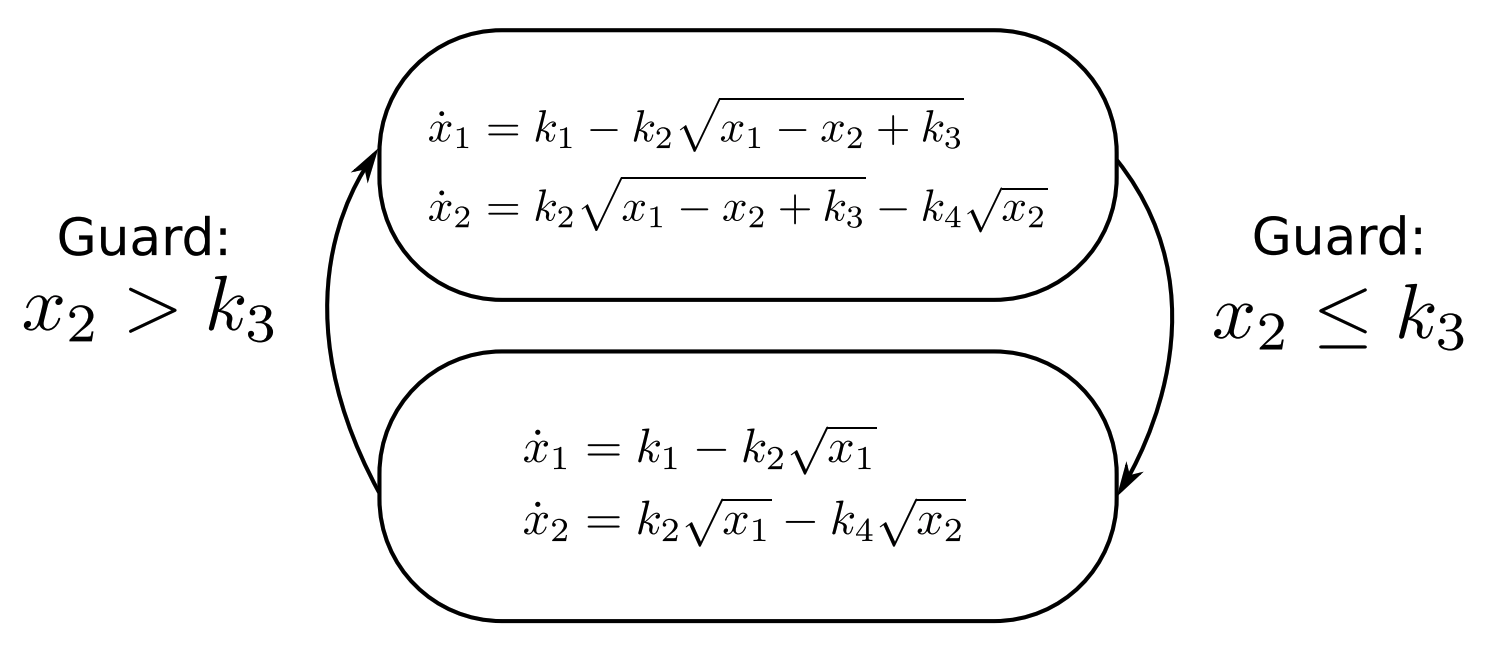
\includegraphics[width=1\linewidth]{./fig/diagrams/two-tank-ha.png}
	  \caption{A single hybrid automaton model}
	\end{subfigure}
	\caption{Two-tank example used in \footfullcite{navarro2016deadness}}
	\label{fig:test}
	\end{figure}
\end{frame}




\begin{frame}[c] \frametitle{ Zero-based guards }
	\vspace{-5pt}
	\begin{block}{Definition}
		A zero-based guard is a constraint expressed in a specific format in Equation~\eqref{eq:zero-based-form}.
		\begin{equation}
			g(X(t), I(t)) \otimes 0, \quad \otimes \in \{<, >, \leq, \geq, == \}
			\label{eq:zero-based-form}
		\end{equation}
		$g(X(t), I(t))$ is called a \emph{guard trace}. Consider it as a signal evolving over time. By abuse of notation, we denote $g(t)$. Naturally, solving it for $t$ gives the values satisfying the guard. 
	\end{block}
	
	\begin{block}{Proposition}
		Any guard can be easily expressed in the zero-based format.\\
		\emph{Proof.} Rearrange the constraint to move everything to the left-hand side.
	\end{block}
	 
	\begin{block}{Example}
		A nonlinear guard: $ 3x + 4xy > (x+1)^2$ \\
		Zero-based form: $ 3x + 4xy - (x+1)^2 > 0$
	\end{block}
\end{frame}

\begin{frame}[c] \frametitle{ Guard-Dependent Dynamic Quantum }
	\begin{block}{Definition: Quantum }
		In QSS, simulation step is invoked based on a signal $x(t)$ and a quantum $\Delta q_x$.
		\begin{equation}
			| x(t) - x(t_0) | = \Delta q_x, \quad \therefore x(t) = x(t_0) \pm \Delta q_x
		\end{equation}
	\end{block}
	
	\begin{block}{ Dynamic Quantum }
		Similar to QSS, we have $g(t) = g(t_0) \pm \Delta q_g$ \\
		We set the quantum based on the guard $\Delta q_g = g(t_0)$\\
		Now, we need to solve:
		\begin{itemize}
			\item $g(t) = 0$, equivalent to solving the guard constraint.
			\item $g(t) = 2 g(t_0)$, when the guard trace moves away from the zero line.
		\end{itemize}	
	\end{block}
\end{frame}

\begin{frame}[c] \frametitle{ Guard-Dependent Dynamic Quantum (Cont.) }
	\begin{figure}
		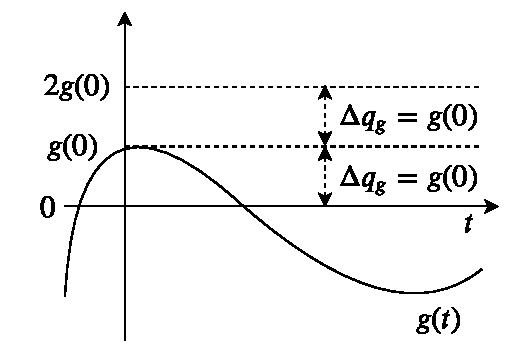
\includegraphics[width=0.7\textwidth]{./fig/diagrams/deltaq.pdf}
	\end{figure}
\end{frame}

\begin{frame}[c] \frametitle{ Taylor expansion of zero-based guards }
	\begin{block}{Description}
		To avoid expensive computation, we want to solve $g(t)$ in polynomial complexity. By abuse of notation, we denote:
		\begin{itemize}
			\item 1st-derivative: $g^{(1)}(t) = \dfrac{d}{dt} \big( g(X(t), I(t)) \big)$
			\item 2nd-derivative: $g^{(2)}(t) = \dfrac{d^2}{dt^2} \big( g(X(t), I(t)) \big)$
		\end{itemize}
		Then, the Taylor polynomials of the guard at time $t_0$ is:
		\begin{equation}
			g(t) = g(t_0) + \mathlarger{\sum}_{n=1}^{\infty} \dfrac{g^{(n)}(t_0)}{n!} \cdot (t - t_0)^n
		\end{equation}
	\end{block}
\end{frame}

\begin{frame}[c] \frametitle{ Theorem: solving a guard always has at least one real root }
	\begin{block}{Lemma}
		Let $0 = a_n x^n + a_{n-1} x^{n-1} + ... + ax \pm c$, be a polynomial of degree $n$ with real coefficients. Then, $f(x)$ has at least one real positive root.
	\end{block}
	\begin{block}{proof}
		Let $m \in \mathbb{Z}^{\geq 0}$ be the number of sign changes within the sequence $(a_n,...,a)$ (i.e., without considering $\pm c$). The possible values of $m \in [0,n-1]$. Descartes' rule of signs states that, if there are $m$ number of sign changes, then there are exactly $m$ real positive roots or less but an odd number of roots. 
		\begin{itemize}
			\item Case $m \geq 1$: regardless of considering the sign of $\pm c$, there is always at least one real positive root by Descartes' rule of signs. 
			\item Case $m = 0$: since $\pm c$ can be either signs, there is always a sign change between $a$ and $c$. Thus, there is at least one real positive root.
		\end{itemize}
	\end{block}
\end{frame}

\begin{frame}[c] \frametitle{ Theorem: solving a guard always has at least one real root (Cont.) }
	\begin{block}{Theorem}
		Let $g(t)$ be a Taylor polynomials of $n$ degree. Then, solving either $g(t) = 0$ or $g(t) = 2g(t_0)$ always result in at least one real positive root.
	\end{block}
	\begin{block}{proof}
		\begin{itemize}
			\item Case $g(t) = 0$: we have $0 = g(t_0) + \mathlarger{\sum}_{n=1}^{\infty} \dfrac{g^{(n)}(t_0)}{n!} \cdot (t - t_0)^n$. 
			\item Case $g(t) = 2g(t_0)$: we have $0 = -g(t_0) + \mathlarger{\sum}_{n=1}^{\infty} \dfrac{g^{(n)}(t_0)}{n!} \cdot (t - t_0)^n$.
		\end{itemize}
		Combining two cases, we have $0 = \pm g(t_0) + \mathlarger{\sum}_{n=1}^{\infty} \dfrac{g^{(n)}(t_0)}{n!} \cdot (t - t_0)^n$. Therefore, the previous Lemma applies directly.
	\end{block}
\end{frame}

\begin{frame}[c] \frametitle{ Finding the first positive real root }
	\begin{algorithm}[H]
	\SetAlgoLined
	\SetKwInOut{Function}{Function}
	\SetKwInOut{Input}{Input}
	\SetKwInOut{Output}{Output}
	\Function{FirstRoot}
	\Input{$\vec{X}$ cont vars smooth tokens, $\vec{I}$ input var smooth tokens, and the guard $g$.}
	\Output{the first root $t_{f}$}
	TaylorCoeff $\leftarrow$ ComputeDerivatives($g(t)$, $\vec{X}$, $\vec{I}$)\;
	Roots $\leftarrow$ Solve(TaylorCoeff)\;
	\ForEach{$r \in $Roots $\wedge$ $r < 0$}{
		Roots.pop($r$)\;	
	}
	$t_f \leftarrow $ min(Roots)\;
	\caption{Computing the first positive real root}
	\end{algorithm}
\end{frame}


\begin{frame}[c] \frametitle{ Approximation validity checking using local truncation error }
	\begin{block}{Local Truncation Error Definition}
		For a signal $x(t)$, let $x^h(t)$ be a precise approximation (i.e., $n$th order), and $x^l(t)$ be a relatively less precise approximation (i.e., $n-1$th order). Then. local truncation error $LTE_x(t)$ is:
		\begin{equation}
			LTE_x(t) = | x^h(t) - x^l(t) |
		\end{equation}
	\end{block}
	\begin{block}{Lemma}
		Local truncation error of the guard $g(t)$ is equivalent to the last term (i.e., highest order) polynomial term. 
		\begin{equation}
			LTE_g(t) = \dfrac{| g^{(n)}(t_0) |}{n!}(t-t_0)^n
		\end{equation}
		If we want to ensure a certain LTE,
		\begin{equation}
			t = \sqrt[n]{\dfrac{LTE \times n!}{ |g^{(n)}(t_0)|}} + t_0
		\end{equation}
	\end{block}
\end{frame}

\begin{frame}[c] \frametitle{ Approximation validity checking using local truncation error (cont.) }
	\begin{block}{proof}
		Consider $n$th order $g(t)$. We have a high and low order approximations: 
		\begin{gather}
			g^h(t) = g(t_0) + \mathlarger{\sum}_{i=1}^{n} \dfrac{g^{(i)}(t_0)}{i!} \cdot (t - t_0)^i \\
			g^l(t) = g(t_0) + \mathlarger{\sum}_{i=1}^{n-1} \dfrac{g^{(i)}(t_0)}{i!} \cdot (t - t_0)^i 	\\			
		\end{gather}
		Therefore, we have:
		\begin{equation}
			LTE_g(t) = | g^h(t) - g^l(t) | = \dfrac{ | g^{(n)}(t_0)|}{n!}(t-t_0)^n		
		\end{equation}
	\end{block}
\end{frame}

\begin{frame}[c] \frametitle{ Computing the step size $\delta$ }
	\begin{algorithm}[H]
	\SetAlgoLined
	\SetKwInOut{Input}{Input}
	\SetKwInOut{Output}{Output}
	\Input{$\vec{X}$, $\vec{I}$, and list of guards $G$}
	\Output{Step size $\delta$}
	$\xi \leftarrow \phi$\;
	\ForEach{ var $\in \vec{X} \cup \vec{I}$}{
		$t_{var} \leftarrow$ ValidTime(var, $k$)\;
		$\xi$.append($t_{var}$)\;
	}
	\ForEach{guard $g$ from the current location}{
		$t_r \leftarrow$ firstRoot($g, \vec{X}, \vec{I}$)\;
		$t_{val}\leftarrow $ ValidTime($g$, $k$)\;
		$t_{grd} \leftarrow$ min($t_r, t_{val}$)\;
		$\xi$.append($t_{grd}$)\;
	}
	$\delta \leftarrow $ min($\xi$)\;
	\caption{ $\delta$ computation }
	\end{algorithm}
\end{frame}

\begin{frame}[c] \frametitle{ Bounded local truncation error }
	\begin{block}{Lemma}
		The local truncation error value is monotonically increasing over time such that for any two time values $t_1$ and $t_2$ such that $t_1 < t_2$, then $LTE(t_1) < LTE(t_2)$ is always true.
	\end{block}
	\begin{block}{proof}
		We can directly prove this by considering $LTE_g(t_2) - LTE_g(t_1) > 0$. \\ 
		Since $LTE_g(t) = \dfrac{|g^{(n)}(t_0)|}{n!}(t-t_0)^n$, \\ 
		$LTE_g(t_2) - LTE_g(t_1) > 0 \implies \dfrac{|g^{(n)}(t_0)|}{n!} \bigg( (t_2-t_0)^n - (t_1-t_0)^n \bigg) > 0 $ \\
		$\because \dfrac{|g^{(n)}(t_0)|}{n!} > 0, \quad (t_2-t_0)^n - (t_1-t_0)^n > 0$ needs to be true. \\
		$t_2 > t_1 > t_0 > 0, \quad \therefore (t_2- t_0) > 0 \wedge (t_1 - t_0) > 0 \wedge (t_2- t_0) > (t_1- t_0)$. \\
		Consequently, $(t_2-t_0)^n - (t_1-t_0)^n > 0$ is always true. \\
		Therefore, $LTE_g(t_2) - LTE_g(t_1) > 0$ is always true.
	\end{block}
	
\end{frame}

\begin{frame}[c] \frametitle{ Bounded local truncation error (cont.) }
	\begin{block}{Theorem}
		The computed $\delta$ at time $t_0$ in Algorithm 2 guarantees, for any state variable $x$, the local truncation error $LTE_x(t)$ is bounded such that $LTE_x(t) \leq k$ is satisfied for $\forall t \in [t_0, t_0 + \delta]$, where $k$ is the user specified constant.
	\end{block}
	\begin{block}{proof}
		Without loss of generality, we assume $t_0 = 0$. For any arbitrarily chosen variable $x$, we have $t_x =$ ValidTime($x$, $k$) in Algorithm 2. Since $\delta$ is assigned to the minimum value, $\delta$ can be either equal to or less than $t_x$.
		\begin{itemize}
			\item Case $t_x = \delta$: $LTE_x(t_x) = k = LTE_x(\delta)$. $\forall t \in [0, \delta]$, by the previous Lemma, $LTE_x(t) \leq LTE_x(\delta)$. Hence, $LTE_x(t) \leq k$.
			\item Case $t_x > \delta$: by the previous Lemma, $LTE_x(\delta) < LTE_x(t_x) = k$ holds. Furthermore, $\forall t \in [0, \delta]$, $LTE_x(t) \leq LTE_x(\delta) < LTE_x(t_x) = k$.
		\end{itemize}
	\end{block}
\end{frame}

\begin{frame}[c] \frametitle{ Simulation Execution Algorithm }
	\begin{algorithm}[H]
	\SetAlgoLined
	\SetKwInOut{Input}{Input}
	\SetKwInOut{Output}{Output}
	\Input{List of HIOA/PDs $Q$, List of connectors $C$}
	\Output{The output traces $Trac$}
	 initialization($Q$)\;
	 $time \leftarrow 0$\;
	 \While{$time \leq T_{max}$}{
	  InterLocation($Q$)\;
	  $Trac$.append($time$, getOutputValues($Q$)\;
	  
	  \lForEach{connector $c \in C$}{ExchangeTokens($c, Q$)}
	  \lForEach{$HIOA^+$ object $q \in Q$}{	  $\delta$.append(ComputeDelta($q$))}

	  $\delta_{step} \leftarrow $ min($\delta$)\;
	  \eIf{ $time + \delta_{step} > T_{max}$ }{
		$time \leftarrow T_{max}$
	  }{
		$time \leftarrow$ time $+ \delta_{step}$
	  }
	  
	 }
	 \caption{Simulation Execution Pseudo Code}
	\end{algorithm}
\end{frame}

%\begin{frame} \frametitle{Supplementary Slides}
\end{frame}

\begin{frame} \frametitle{RK45 Formula}
	\centering
	\begin{figure}
		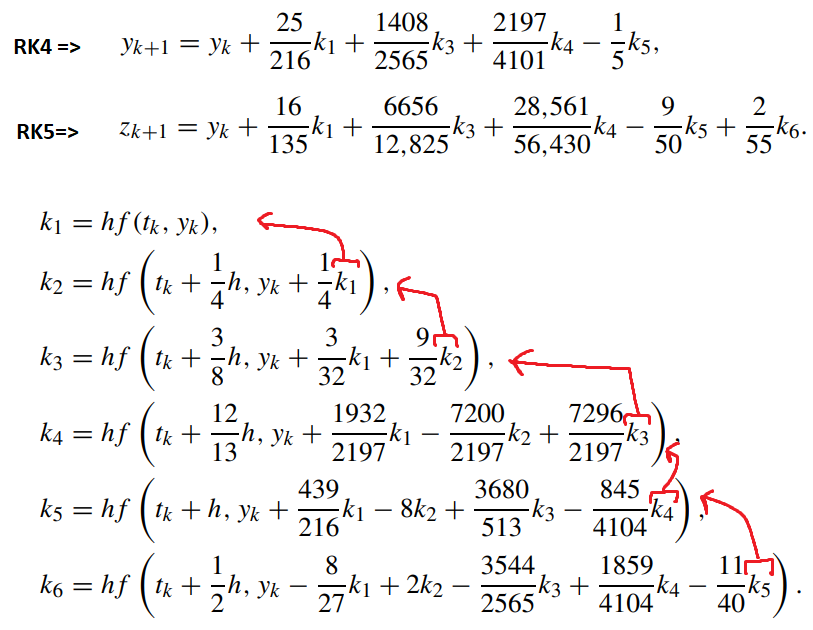
\includegraphics[width=0.8\textwidth]{./fig/rk45.png}
	\end{figure}
\end{frame}


\begin{frame}[c] \frametitle{ Syntax changes to allow smooth-token calculation }
	\begin{block}{Description}
		\begin{itemize}
			\item To allow calculation of smooth-token of higher than 1st order, we need more differential equation information.
		\end{itemize}
	\end{block}
	\begin{block}{Changes}
		\begin{itemize}
			\item The vector field $f$ definition is changed to indicate the differentiation order.
			\begin{itemize}
				\item $f : \mathbf{L} \times 2^X \times 2^I \times \mathbb{N}_{\geq 1} \rightarrow \mathbb{R}^n$.
				\item E.g., $f(l,\overrightarrow{x}, \overrightarrow{i}, 2) = x_i^{(2)}$.
			\end{itemize}
			\item The vector field $h$ definition is changed to indicate the differentiation order.
			\begin{itemize}
				\item $h : \mathbf{L} \times 2^X \times 2^I \times \mathbb{N}_{\geq 0} \rightarrow \mathbb{R}^n$.
				\item E.g., $h(l,\overrightarrow{x}, \overrightarrow{i}, 3) = o_i^{(3)}$.
			\end{itemize}
		\end{itemize}
	\end{block}
\end{frame}

\begin{frame}[c] \frametitle{ Smooth-token Calculation / Exchange }
	\begin{block}{Proposition}
		\begin{myitemize}
			\item The $(m+1)$th differential equations in QSHIOA are always depends on lower order values up to $m$.
			\item E.g., we have a coupled ODEs, $\dot{x} = xy$ and $\dot{y} = y - x$.
			\item $\ddot{x} = \frac{dx}{dt} y + x \frac{dy}{dt} = \dot{x}y + \dot{y}x$, $\quad \ddot{y} = \dot{y} - \dot{x}$.
			\item $\dddot{x} = \ddot{x}y + 2\dot{x}\dot{y} + \ddot{y}x$, $\quad \dddot{y} = \ddot{x} - \ddot{y}$.
		\end{myitemize}
	\end{block}
	\begin{block}{Calculation Dependency}
		\begin{itemize}
			\item From the proposition, the calculation of any $(m+1)$th order ODE depends on the values of $m$th order.
			\item So, there is a dependency.
		\end{itemize}
	\end{block}
\end{frame}

\begin{frame}[c] \frametitle{Overcoming the stationary point execution inefficiency}
	\begin{block}{Cause}
		\begin{itemize}
			\item The rate of change is almost zero due to the extremely small/zero gradient.
			\item Many iterations are needed to narrow down to the point where the approximations intersect with the $\Delta q$ threshold.
		\end{itemize}
	\end{block}
	\begin{block}{Proposing approach}
		\begin{itemize}
			\item When we reach the maximum iteration depth, and still could not reach narrow enough, we need to somehow force move the time.
			\item Current implementation has a configuration parameter called $escape_time$, which is a fixed value.
			\item Since we have the guards already in Taylor polynomials, we should be able to use the error estimation formula (remainder theorem -- Lagrange formula). 
			\item $R(t) = \frac{f^{(n+1)}(c)}{(n+1)!}t^{(n+1)}$
			\item Where, $c$ is a value between $(0, t)$. It is important that this is an open interval!
		\end{itemize}
	\end{block}
\end{frame}

\begin{frame}[c] \frametitle{Result Section}
	\begin{block}{What are we going to show?}
		\begin{itemize}
			\item We are going to show the comparison of three methods:
			\begin{enumerate}
				\item RK45: this will be used from Simulink/Stateflow.
				\item MQSS: Although the proof is not for multivariate functions, MQSS still can be executed.
				\item Proposed one.
			\end{enumerate}
		\end{itemize}
	\end{block}
\end{frame}

\begin{frame}[c] \frametitle{ Recap: Quantised State Hybrid Input Output Automata (QSHIOA) }
	\begin{block}{Definition}
		$\mathcal{H}_{q} = \langle L, X, X_q, V, O, Init, f, f_q, h, Inv, E,
		  G, R\rangle $
		\begin{itemize}
		\item $L = \{l_{0},\ldots,l_{n}\}$ a set of discrete locations.
		\item $V$ is a finite collection of input variables.
		\item $O$ is a finite collection of output variables.
		\item $X$ is a finite collection of continuous variables.
		\item $Init \subseteq \{l_0\} \times \mathbf{X} \times \mathbf{O}$.
		\item $f : \mathbf{L} \times \mathbf{V} \times \mathbf{X} \rightarrow \mathbb{R}^{n}$ is ODE, e.g., $f(l, i, x)$ and $f_{q}(l, i, x_{q})$.
		\item $h : \mathbf{L} \times \mathbf{X} \rightarrow \mathbf{O}$.
		\item $Inv: \mathbf{L} \rightarrow 2^{\mathbf{X} \times \mathbf{V} }$
		\item $E \subset \mathbf{L} \times \mathbf{L} $ is a collection of discrete edges.
		\item $G : E \rightarrow 2^{\mathbf{X} \times \mathbf{V}}$ assigns to each
		  $e = (l, l') \in E$ a guard.
		\item
		  $R : E \times \mathbf{X} \times \mathbf{V} \rightarrow 2^{\mathbf{X} \times \mathbf{O}}$
		  assigns to each $e = (l,l') \in E$.
		\end{itemize}
	\end{block}
\end{frame}

\begin{frame}[c] \frametitle{Algorithm Inefficiency Near Stationary Points}
	\centering
	\begin{figure} 
		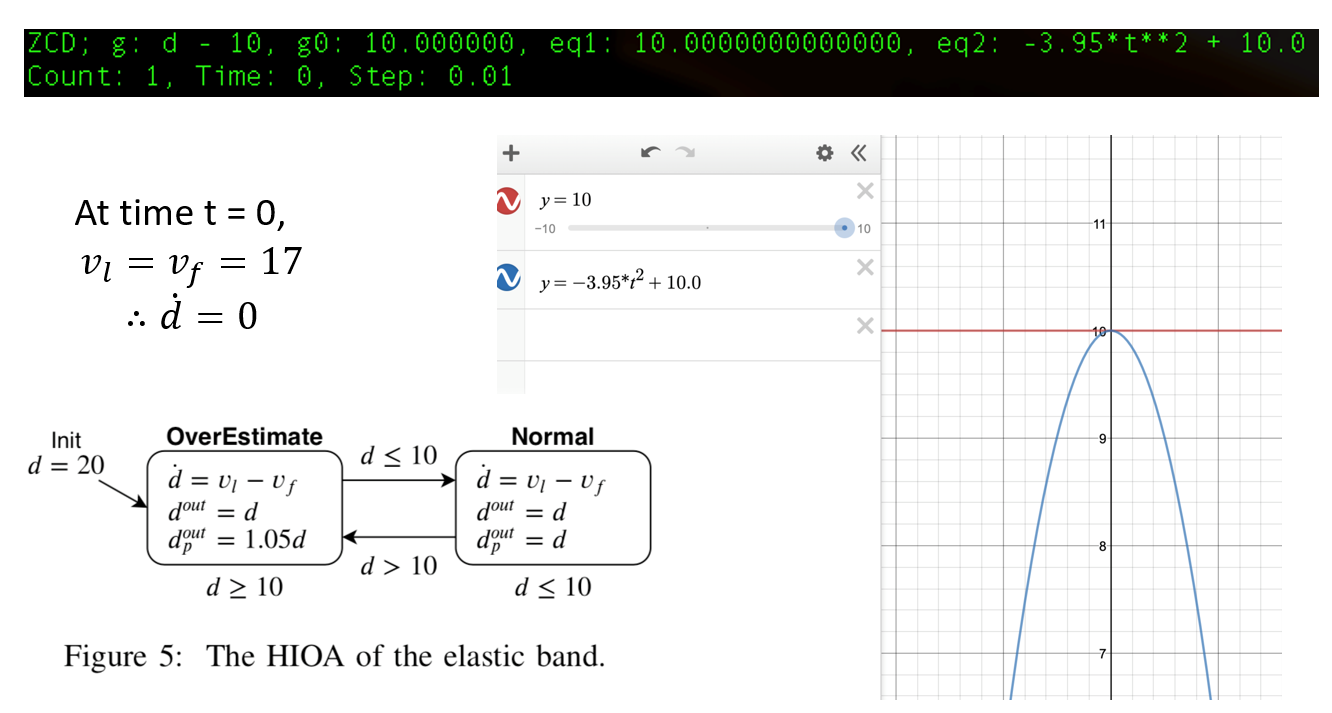
\includegraphics[width=1\textwidth]{./fig/inefficiency.png}
	\end{figure}
\end{frame}

\begin{frame} \frametitle{Results}
	\begin{table}[]
		\begin{tabular}{ccc}
			\toprule
			Criteria 	    & Proposed & MQSS12 	\\ \midrule
			Step count      & 	185		&  1548 	\\
			Execution time  &   3.163    & 85.0442  \\
			Mean step size  &	0.10811  & 0.01292  \\
			Correlation     &   0.9999   & 0.9999   \\ \bottomrule
		\end{tabular}
		\caption{Cooperative Robot System Benchmark }
	\end{table}
	
	\begin{table}[]
		\begin{tabular}{ccc}
			\toprule
			Criteria 	    & Proposed & MQSS12 	\\ \midrule
			Step count      & 	2690	&  4840 	\\
			Execution time  &   205.231  & 4257.335  \\
			Mean step size  &	0.0223  & 0.0124  \\
			Correlation     &   0.9996   & 0.9604   \\ \bottomrule
		\end{tabular}
		\caption{Collision Avoidance System Benchmark }
	\end{table}
\end{frame}



%Include your other sections
%\begin{frame} \frametitle{Results}
	\begin{table}[]
		\begin{tabular}{ccc}
			\toprule
			Criteria 	    & Proposed & MQSS12 	\\ \midrule
			Step count      & 	185		&  1548 	\\
			Execution time  &   3.163    & 85.0442  \\
			Mean step size  &	0.10811  & 0.01292  \\
			Correlation     &   0.9999   & 0.9999   \\ \bottomrule
		\end{tabular}
		\caption{Cooperative Robot System Benchmark }
	\end{table}
	
	\begin{table}[]
		\begin{tabular}{ccc}
			\toprule
			Criteria 	    & Proposed & MQSS12 	\\ \midrule
			Step count      & 	2690	&  4840 	\\
			Execution time  &   205.231  & 4257.335  \\
			Mean step size  &	0.0223  & 0.0124  \\
			Correlation     &   0.9996   & 0.9604   \\ \bottomrule
		\end{tabular}
		\caption{Collision Avoidance System Benchmark }
	\end{table}
\end{frame}



%\section{Whatever}
%\input{parts/whatever}

%Don't change: this automagically creates the reference slides
\begin{frame}[t,allowframebreaks]{References} %% Aligned top
	\printbibliography
\end{frame}

\appendix

%Include any appendix slides beyond here

\end{document}